\documentclass{beamer}
\usepackage[utf8]{inputenc}

\usetheme{Madrid}
\usecolortheme{default}
\usepackage{amsmath,amssymb,amsfonts,amsthm}
\usepackage{txfonts}
\usepackage{tkz-euclide}
\usepackage{listings}
\usepackage{adjustbox}
\usepackage{array}
\usepackage{tabularx}
\usepackage{gvv}
\usepackage{lmodern}
\usepackage{circuitikz}
\usepackage{tikz}
\usepackage{graphicx}

\setbeamertemplate{page number in head/foot}[totalframenumber]

\usepackage{tcolorbox}
\tcbuselibrary{minted,breakable,xparse,skins}



\definecolor{bg}{gray}{0.95}
\DeclareTCBListing{mintedbox}{O{}m!O{}}{%
  breakable=true,
  listing engine=minted,
  listing only,
  minted language=#2,
  minted style=default,
  minted options={%
    linenos,
    gobble=0,
    breaklines=true,
    breakafter=,,
    fontsize=\small,
    numbersep=8pt,
    #1},
  boxsep=0pt,
  left skip=0pt,
  right skip=0pt,
  left=25pt,
  right=0pt,
  top=3pt,
  bottom=3pt,
  arc=5pt,
  leftrule=0pt,
  rightrule=0pt,
  bottomrule=2pt,
  toprule=2pt,
  colback=bg,
  colframe=orange!70,
  enhanced,
  overlay={%
    \begin{tcbclipinterior}
    \fill[orange!20!white] (frame.south west) rectangle ([xshift=20pt]frame.north west);
    \end{tcbclipinterior}},
  #3,
}
\lstset{
    language=C,
    basicstyle=\ttfamily\small,
    keywordstyle=\color{blue},
    stringstyle=\color{orange},
    commentstyle=\color{green!60!black},
    numbers=left,
    numberstyle=\tiny\color{gray},
    breaklines=true,
    showstringspaces=false,
}
%------------------------------------------------------------

\title
{4.12.8}
\date{September 5,2025}
\author 
{AI25BTECH11003 - Bhavesh Gaikwad}



\begin{document}


\frame{\titlepage}
\begin{frame}{Question}
Distance of the point $(\alpha, \beta, \gamma)$ from y-axis is\\
a) $\beta$\\
b) $|\beta|$\\
c) $|\beta + \gamma|$\\
d)$\sqrt{\alpha^2 + \gamma^2}$ \\
\end{frame}


\begin{frame}[fragile]
    \frametitle{Theoretical Solution}
Let $\vec{A} = \myvec{\alpha \\ \beta \\ \gamma}$\\ 
Let $\vec{B}$ be an arbitrary point on the y-axis.

\begin{equation}
    \text{Equation of y-axis: } \vec{r} = t\vec{e_2} \, \,
    OR \, \, \vec{r}=t\myvec{0 \\ 1 \\ 0}
\end{equation}

\begin{equation}
\therefore \, \vec{B}=\myvec{0 \\ t \\0}
\end{equation}

\begin{equation}
\text{For minimum distance from y-axis: } \vec{(A-B)} \text{ should be perpendicular to } \vec{e_2}
\end{equation}

\begin{center}
    OR
\end{center}

\end{frame}

\begin{frame}[fragile]
\frametitle{Theoretical Solution}

\begin{equation}
\vec{(A-B)}^T\vec{e_2} =0 \, \Rightarrow \, \myvec{\alpha \\ \beta-t \\ \gamma}^T\myvec{0 \\ 1 \\ 0} = 0     
\end{equation}\\

Therefore, from Equation 4,
\begin{equation}
t=\beta
\end{equation}

Therefore the distance between y-axis and $\vec{A}$ is:
\begin{equation}
    \norm{\vec{B-A}}  = \norm{\myvec{\alpha \\ 0 \\ \gamma}} = \sqrt{\alpha^2 + \gamma^2}
\end{equation}

\begin{equation}
\boxed{\text{Therefore, Option D is Correct.}}    
\end{equation}
\end{frame}


\begin{frame}{Image}
   \centering
    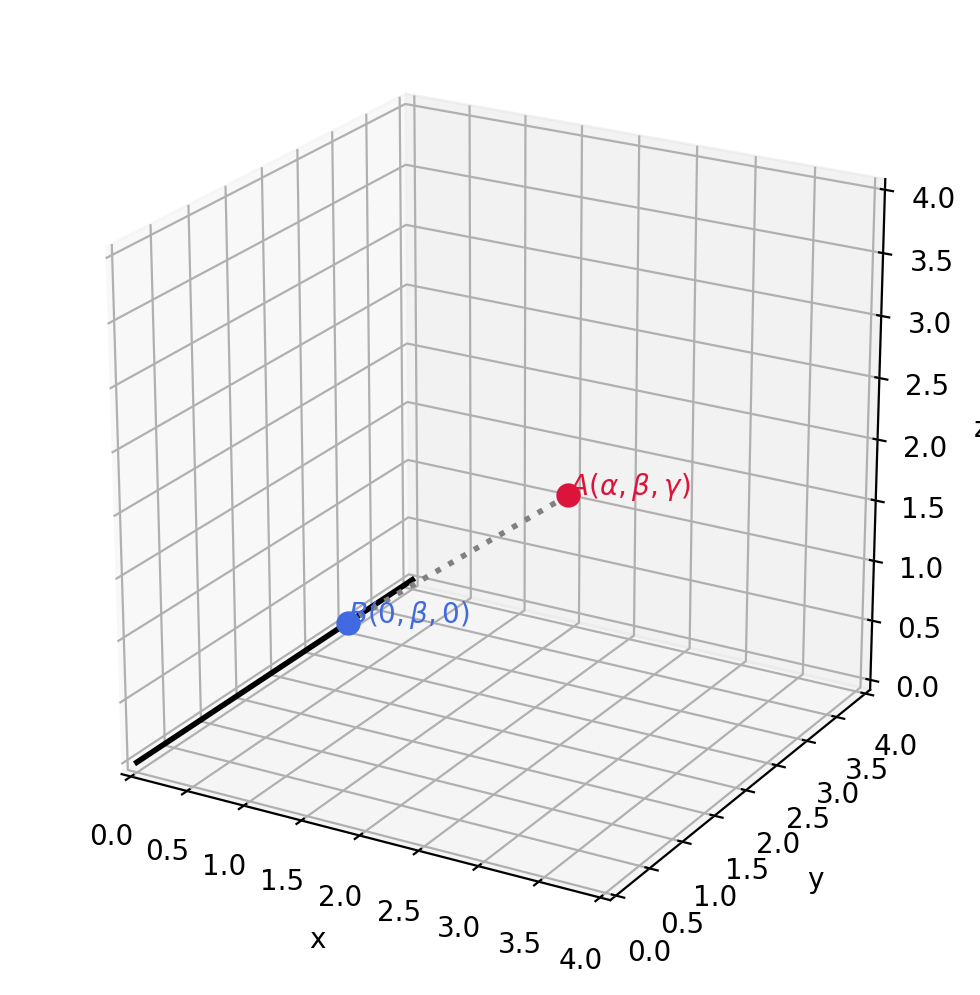
\includegraphics[width=\columnwidth, height=0.8\textheight, keepaspectratio]{figs/fig1.png}
    \label{fig:Beamer/figs/fig1.png}
\end{frame}


\end{document}